\documentclass[a4paper,parskip,headheight=38pt]{scrartcl} % article or scrartcl
\usepackage[utf8]{inputenc}
\usepackage[T1]{fontenc}
\usepackage{amsmath,amssymb,amsfonts}
\usepackage[%
  automark,
  headsepline                %% Separation line below the header
]{scrlayer-scrpage}
\usepackage[english]{babel}
\usepackage{hyphenat}
\usepackage[hidelinks]{hyperref}
\usepackage[top=1.4in, bottom=1.5in, left=1in, right=1in]{geometry}
\usepackage{lastpage}
\usepackage{csquotes}
\usepackage{microtype}
\usepackage{datetime}

\usepackage{url}

\usepackage{todonotes}

\usepackage[normalem]{ulem}
\usepackage{enumerate}
\usepackage{hyperref}
\usepackage{csvsimple}

\usepackage{microtype}

\usepackage[hang]{footmisc}
\setlength{\footnotemargin}{3mm}

\usepackage{enumitem}

\usepackage{color}

\usepackage[export]{adjustbox}

\newcommand*{\rom}[1]{\uppercase\expandafter{\romannumeral #1\relax}}

% \usepackage{multicol}
\usepackage{graphicx}
\usepackage{graphics}
% \usepackage{float}
% \usepackage{caption}

\parindent 0pt
\parskip 6pt

\clubpenalty = 10000
\widowpenalty = 10000
\displaywidowpenalty = 10000

\setkomafont{pagehead}{\normalfont\sffamily\footnotesize}
\addtolength{\headheight}{+13pt}
\lohead{Marlene Böhmer, s9meboeh@stud.uni-saarland.de, 2547718 \\
	Maximilian Köhl, s8makoeh@stud.uni-saarland.de, 2553525 \\
	Maximilian Schwenger, schwenger@stud.uni-saarland.de, 2542438\\
	Ben Wiederhake, s9bewied@stud.uni-saarland.de, 2541266}
\rohead{\includegraphics[height=36pt, right]{../logo/logo.png} \newline ES16, Verification Document, Group 6, Page {\thepage}/{\pageref*{LastPage}}}

\newtimeformat{mytime}{\twodigit{\THEHOUR}\twodigit{\THEMINUTE}\twodigit{\THESECOND}}
\settimeformat{mytime}
\newdateformat{mydate}{\twodigit{\THEYEAR}\twodigit{\THEMONTH}\twodigit{\THEDAY}}
\cfoot{\tiny\texttt{ID \mydate\today\currenttime}}
\chead{} % Needed because now the \subsections get displayed
\pagestyle{scrheadings}

% \renewcommand{\headrulewidth}{0pt}
% \addtolength{\textheight}{+30mm}
% \addtolength{\textwidth}{+50mm}
% \addtolength{\hoffset}{-7mm}

% \newcommand{\Omicron}{\ensuremath{\mathcal{O}}}
% \newcommand{\omicron}{\ensuremath{o}}
% \newcommand{\set}[1]{\{#1\}}
% \newcommand{\abs}[1]{\lvert #1 \rvert}

\DeclareMathOperator{\sinc}{sinc}

\newcommand{\incomplete}[1]{\textless{} #1 \textgreater{}}

\newcommand{\teststrat}[5]{
    \subsubsection{Test Strategy}
	\textbf{Component:} #1 \\
	\noindent\textbf{What should be tested?} \\
    \noindent #2 \\
	\noindent\textbf{How can it be tested?} \\
    \noindent\textcolor{blue}{Setup:} #3 \\
    \noindent\textcolor{blue}{Applicable Techniques:} #4 \\
	\noindent\textbf{What cannot be tested? Why?} \\
    \noindent #5
}

\newcommand{\testprot}[6]{
    \subsubsection{Test Protocol}
    \textbf{Component:} #1 \\
    \noindent\textbf{What should be tested?} \\
    \noindent #2 \\
    \noindent\textbf{How can it be tested?} \\
    \noindent\textcolor{blue}{Setup:} #3 \\
    \noindent\textcolor{blue}{Applicable Techniques:} #4 \\
    \noindent\textbf{What cannot be tested? Why?} \\
    \noindent #5
    \noindent\textbf{Results:} \\
    \noindent #6
}

\newcommand{\ie}{i.e.}

\newcommand{\BLACK}{\textbf{Integration test: }}
\newcommand{\WHITE}{\textbf{Unit test: }}

\newcommand{\mics}{$\mu$s}

\begin{document}

\section{Overview}

On a grand scheme the software is divided into the following subcomponents:

\begin{itemize}
	\item Controller
	\item Traffic Cop Eyes
	\item Blind Traffic Cop 
	\item RHR
	\item Victim Direction\footnote{We will present a test protocol
   for this component.}
	\item Victim Finder
	\item Path Finder
	\item Path Executor
	\item Pickup Artist
    \item Approximator
    % \item Proximity Map
    % \item Proximity Filter
\end{itemize}

Each of those components is subject of one or more test strategies either for
the whole component at once, or their subcomponents separately.
\subsection{Controller}
\subsubsection{Purpose}
	Connects each component's inputs and outputs. Steps appropriate components
    based on the Blind Cop's output. This component does not incorporate further
    logic.
\teststrat{Controller}{
    The correct connection between the Tin Bot's different subcomponents, \ie,
    the correct overall behavior for a single Tin Bot without taking any T2T
    connection into account.
}{
    Maze, Victim, one Tin Bot including all LEDs, LPS, debug monitor.
}{
    \BLACK Setup the maze. Place the victim and the Tin Bot inside
    appropriately. Setup
    the LPS and make sure that a Bluetooth connection between the LPS, the Tin
    Bot, and the debug monitor is established. Turn on the E-Puck and evaluate
    the behavior based on movements and visual feedback by the LEDs.
}{
    Correctness of subcomponents separately is not tested, because they are
    covered in other, more appropriate test cases. Moreover, the T2T connection
    is not tested for the same reasoning.
}
%
\subsection{Traffic Cop Eyes}
\subsubsection{Purpose}
The Traffic Cop Eyes component observes IR-Sensor data and decides when it is a
good idea to start the Victim Direction component. This decision is forwarded to
the Blind Cop, which makes a final decision.
\teststrat{Traffic Cop Eyes Full}{
    Correct behavior based on given unstabilized sensor data. 
}{
    Part \rom{1}: MatLab, compiled code. Part \rom{2}: Full Setup, \ie, LPS,
    victim, Tin Bot(s), debug monitor, maze.
}{
    Part \rom{1}: \BLACK Run the test cases from the virtual prototype, but use
    actual
    compiled code instead of the Simulink model. Check for correctness based
    on the output. \\
    Part \rom{2}: \BLACK Run full process, check for ignorance towards incoming
    signals
    even though the intended behavior dictates a reaction. 
}{
    There are no unit tests for this component due to its importance and
    simplicity. So bugs are unlikely and close to impossible to remain
    unnoticed.
}

\teststrat{Victim Directing Start}{
    When a signal from the victim is received, the Victim Direction component
    is supposed to be started, but only after having traveled an appropriate
    amount
    of time, another measurement should be initiated.
}{
    Victim, maze, LPS, Tin Bot.
}{
    \BLACK Setup the maze as well as the LPS. Place the victim and the
    Tin Bot in the
    maze and turn them on. Wait for the Tin Bot to receive a signal and check
    for the component's signature movement, \ie, turning a full circle.

    Wait for the second measurement to be fully performed, then turn off the Tin
    Bot and measure the traveled distance.
}{
    The correctness of the signals and the output are not tested, because they
    are subject of their own test cases.
}
%
\subsection{Blind Traffic Cop:}
\subsubsection{Purpose}
An arbiter for the subcomponents. It does not take sensor data into account but
relies on other component's outputs for the decision.
\teststrat{Blind Traffic Cop}{
    Correct arbitration of the access to the motors.
}{
    Full Setup.
}{
    \BLACK Each component has a signature behavior and
    their distinction is clear, so a conflict or an incorrect arbitration can be
    spotted easily.
}{
    It is not tested, whether the Controller actually uses the Blind Cop's
    output or decides on its own. If it were so the Tin Bot's behavior would be
    spurious, or correct. In the latter case, we would assume the Blind Cop to
    be correct, even though it is not used at all.
}
%
\subsection{Right-Hand Rule}
\subsubsection{Purpose}
Implementation of the right-hand rule\footnote{For a detailed description,
please see 
\url{https://en.wikipedia.org/wiki/Maze_solving_algorithm\#Wall_follower}
}.
\teststrat{Right-Hand-Rule Obedience}{
    The Tin Bot is supposed to walk straight until sensing a wall. Then, it
    should follow it having the wall on its right-hand side.
}{
    Tin Bot, LPS, debug monitor, maze.
}{
    \BLACK Setup the LPS and the maze. Place a single Tin Bot in the maze and
    turn it
    on. Start the Tin Bot and wait an appropriate amount of time based on the
    maze's layout.

    Check debug data for disagreements with the intended behavior.
}{
    Collision avoidance is not tested on a detailed level, i.e. scraping along
    the wall will not be detectable. This, however, is subject of a dedicated
    test.
}
%
\subsection{Victim Finder}
\subsubsection{Purpose}
Manages gathered data about the victim, i.e. discards old information.

\teststrat{Victim Finder}{
    The Victim Finder should triangulate the victim's position correctly based
    on artificial sample measurements.
}{
    Compiled code.
}{
    \WHITE Run the unit tests and check for failing assignments. 
}{
    Measurements are not tested for sanity, e.g.\ inconsistencies. Results of
    such measurements are not tested.
}

\subsection{Victim Direction}
\subsubsection{Purpose}
Rotates the E-Puck for a full revolution and computes angle/position to the
victim.
\testprot{Victim Direction Computation}{
    Victim Direction is supposed to approximate the normalized angle from its
    current position to the victim. The computation's correctness is tested
    here.
}{
    Part \rom{1}: MatLab, compiled code.
    Part \rom{2}: LPS, debug monitor, Tin Bot, victim.
}{
    Part \rom{1}: \BLACK Start test case from virtual prototype in MatLab, but
    use
    compiled code
    instead of Simulink model. Check the output.
    Part \rom{2}: \BLACK Setup the LPS, place and turn on the Tin Bot as well as
    the
    victim. Make sure a Bluetooth connection between the debug monitor, the Tin
    Bot, and the LPS has been established. 

    Run the Tin Bot, wait until a measurement has been completed, and the result
    has been sent to the debug monitor. Check for approximative correctness.
}{
    Bluetooth connection and correctness of signals are not tested. The former
    one is assumed to be correct, the latter one is subject to its own test
    cases.
}{
    The computed values differ significantly from the actual angles (Figure \ref
    {fig:vddatabad}). As reason we identified reflections caused by the
    environment. To circumvent the problem, we covered the boundary in cellular
    rubber. This should prevent most reflections. Re-running the experiment
    revealed that now the measurement are significantly better (Figure \ref
    {fig:vddatagood}). Most notably, the scattering decreased from $\approx 1.5$
    to $\approx 0.3$.
}

\begin{figure}[t]
\includegraphics[width=\textwidth]{victimdirectionbadplot.pdf}
\caption{Data obtained by running Victim Direction. Reference data was computed
based on a bird's eye view image. Plot shows histogram of deviation from
measured data to the reference value.}
\label{fig:vddatabad}
\end{figure}
\begin{figure}[t]
\includegraphics[width=\textwidth]{victimdirectiongoodplot.pdf}
\caption{Data obtained by running Victim Direction. Reference data was computed
based on a bird's eye view image. The plot shows histogram of deviation from
measured data to the reference value.}
\label{fig:vddatagood}
\end{figure}

\subsection{Path Finder}
\subsubsection{Purpose}
Computes a path from the current position to a goal distance given by the Blind
Traffic Cop based on the internal map. This map consists of data gathered via
proximity sensors and other Tin Bot's broadcasts.

The given goal can be either the victim's position or the initial position, \ie,
the exit.
\teststrat{Path Finder State Machine}{
    The Path Finder should output a given solution path in the correct order and
    raise a flag for the penultimate and last waypoint respectively.
}{
    MatLab, compiled code.
}{
    \BLACK Start the MatLab test case from the virtual prototype using
    the compiled code instead of the Simulink model. Check the outputs.

    Additionally, run the unit tests and check for failing assignments.
}{
    Sanity of given path and especially the finiteness thereof is not tested.
    This is part of a different test.
}

\teststrat{Path Finder Search Algorithm}{
    An promising path based on the internal map should be found while the memory
    needed should be bounded statically.
}{
    Compiled code.
}{
    Unit tests check correctness. Static checks ensure memory bound.
}{
    The behavior for invalid input maps is not tested.
}

\subsection{Path Executor}
Moves the Tin Bot to a given position minding the walls.
\teststrat{Path Executor}{
    A given waypoint should be reached by the Tin Bot using a straight line
    path. If there is an obstacle blocking the way, the Tin Bot should stop.
    Additionally, if the appropriate flag is set, the Path Executor should turn
    the Tin Bot by $180\deg$ and reach the way point in the reverse gear.
}{
    Tin Bot, LPS, walls.
}{
    \BLACK After receiving any valid waypoint, the Tin Bot should
    only stop if the waypoint or a wall is reached. Turn sequence should be
    initiated if the flag is set.
}{
    The invalidity of a waypoint is not checked explicitly. If the point is
    unreachable, the Tin Bot will stop in front of the boundary as if it was a
    wall.
}

\subsection{Pickup Artist}
\subsubsection{Purpose}
Allows robustness against inaccuracies in the victim's computed position by
initiating a small scale search after reaching the expected position.
\teststrat{Pickup Artist}{
    If the victim's position differs from the computed one, the Tin Bot is
    supposed to continue driving towards it until the victim is picked up. If
    the difference is too large, the Tin Bot is supposed to shut down.
}{
    Compiled code.
}{
    % \BLACK Setup LPS, turn on the Tin Bot and the victim. Give the
    % \emph{last} waypoint which is differing slightly from the victim's actual
    % position. The waypoint has to be the last one to ensure that the Tin Bot
    % will be in the right position to initiate the pick up process. Check if the
    % pickup succeeds.

    % Afterwards, the last waypoint is sent while the victim is entirely out of
    % reach. 15 seconds after reaching the waypoint, a full shutdown is expected.

    The unit test ensures that state transitions are taken appropriately.
    This especially means that the Tin Bot shuts down if needed.
}{
    Walls behind the victim's expected position will not be detected. Therefore,
    there is no point in testing for such a behavior.
}

\subsection{Collision Avoidance}
\subsubsection{Purpose}
When the Tin Bot moves too close to a wall, independent of the current mode, it
should stop before any collision takes place.
\teststrat{Collision Avoidance}{
    None of the walls, neither formerly known ones, nor newly added ones, may be
    knocked over.
}{
    Maze, LPS, Tin Bot.
}{
    \BLACK Run different modes in different settings and make sure no
    wall is knocked over.
}{
    Correct overall behavior, because this is subject of own test strategies.
}

% \subsection{Arbiter}
% \subsubsection{Purpose}
% The Tin Bot's position is computed by the approximator based on the data sent to
% the motors. Due to
% slight differences between theory and practice, the computed data might deviate
% from the actual position. For this reason, the LPS sends more precise position
% data. 
% \teststrat{Necessity of the LPS and Quality of the Approximator}{
%     The Tin Bot's position should not change when turning in circles. This,
%     however, is not the case in practice. So the approximator's computed data is
%     compared against the actual position after performing 50 full turns. If the
%     deviation is too high, the necessity of the LPS is confirmed.
% }{
%     Tin Bot, LPS.
% }{
%     \BLACK The Tin Bots rotates for 50 full turns. Afterwards, the traveled
%     distance is measured.
% }

% DEEMED TOO FAR OFF REALITY:
% \subsection{Proximity Map}
% When a Tin Bot walks around, it gathers data about the map using its proximity
% sensors. This data, however, should not be included in internal map
% representation right away. The data is broadcast to all Bots, including
% itself. Using this technique, the latest gathered data is included in the
% internal map independent of whether the Bot gathered the information itself, or
% received it from other ones.

\section{Hardware} 
The hardware is divided into two parts: The environment, and the connection
between the main components, \ie, the Raspberry Pi, and the E-Puck. 
The connection between the components and their respective sensors and actuators
is verified using the following test strategies.

\subsection{Connection Extension Board to E-Puck}

\teststrat{Custom Extension Board Connection Frequency}{
    We guarantee a real time upper bound on the frequency in which sensor data
    is received and can then be processed. The time between two received
    sensor data packages is less than 51ms.

    We test the frequency in which data is received and computed the maximal
    time needed for all interrupt service routine (ISR) to run through, such
    that the
    stated frequency can be guaranteed.
}{
    Oscilloscope, custom extension board, E-Puck.
}{
    We directly measure the signals from the extension board sent using the
    I\textsuperscript{2}C protocol. We send signals to an IR-Sensor to see
    whether the received signal is correct.

    This way we measured that a signal is sent after at most 50ms. 

    The maximal time needed by the interrupt service routines can be obtained by
    computing the schedule for the worst case behavior of the interrupts. For
    this we consider all ISRs, which are scheduled preemptively based on
    static priorities.

    There are five ISRs, ordered by their descending priority:
    \begin{description}
        \item[Timer] The timer ISR is a scheduler for tasks $J^T_i$ concerning
            e.g.\ motor control and internal time. It also sets the start
            condition for the I\textsuperscript{2}C protocol.\\
            \begin{center}
            \begin{tabular}{c | l | r | r}
                $i$ & Task & $T^T_i$ & $C^T_i$ \\
                \hline
                1 & RMotorTimer         & 1,000\mics     & 4\mics \\
                2 & LMotorTimer         & 1,000\mics     & 4\mics \\
                3 & UpdateExtData       & 5,000\mics     & 1\mics \\
                4 & ResetLoopCounter    & 1,000,000\mics & 1\mics \\
                5 & SendHeartBeat       & 1,000\mics     & 10\mics \\
                6 & TinTime             & 1,000\mics     & 1\mics \\
                7 & Timeout             & 100,000\mics   & 1\mics \\
            \end{tabular}
            \end{center}
            Therefore, the timer interrupt needs at most $C_{\text{timer}}
            = \sum_{i = 1}^{7}C^T_i = 22$\mics.

        \item[RX] Receives Bluetooth packets with a period of $\geq$8.6\mics\ 
        and a computation time of 4\mics. However, when a whole map update is
        received, the ISR performs a costly merge operation, which takes
        110\mics. This, however, can only happen every 1000\mics. This is
        guaranteed by the LPS. Moreover, we
        guarantee that after a fully sent message, there is at least 2ms where
        no further message is sent.
        \item[I\textsuperscript{2}C] The data given from the IR-Sensors is copied into local
        memory and can therefore not be lost anymore.

        This process happens in three steps, each of which requires a
        certain downtime in-between. In the first step, the read address is
        written on the bus,
        in the second step a read request is issued, and in the third step the
        received data is written in local memory. 

        After those steps the software can access the data, while in a fourth
        and fifth step the bus is freed and the internal state machine is reset,
        respectively.
        \item[ADC] The analog proximity sensor data is converted into digital
        data.
        \item[TX] Packets are transmitted over Bluetooth.
    \end{description}
    The task information is thusly:
    \begin{center}
    \begin{tabular}{l | r | r}
        Interrupt & $T_{\text{name}}$ & $C_\text{name}$ \\
        \hline
        Timer    & 100\mics       & 4\mics \\
        RX       & 1,000\mics     & 4\mics \\
        I\textsuperscript{2}C      & 5,000\mics     & 1\mics \\
        ADC      & 1,000,000\mics & 1\mics \\
        TX       & 1,000\mics     & 10\mics \\
    \end{tabular}
    \end{center}
    In the resulting worst case schedule, the timer is scheduled and takes up to
    26\mics. Afterwards, the RX ISR can be started taking 110\mics\  for a map
    merge, and 4\mics\  for the normal interrupt. During this process, another
    Timer release time is reached, so the RX is interrupted for 26\mics.
    Consequently, RX finishes after 166\mics.

    Then, the first I\textsuperscript{2}C step takes place, taking 1\mics. From now on, we have to
    wait 80\mics\  in which other interrupts and software steps can take place.
    We ignore all of them if they have a lower priority. Therefore, at time
    200\mics, another Timer ISR is executed, and at time 247 the second I\textsuperscript{2}C step
    takes place taking 1\mics. 

    Now, 160\mics\  have to pass until the third step can take place. At
    time 300\mics\  and 400\mics, another Timer step takes place until at time
    426 the third I\textsuperscript{2}C step is executed taking 5\mics, \ie, the response time for
    having the data in local memory is 431\mics.

    Additionally, when working on volatile data, we disable interrupts until the
    operation has finished. We can guarantee that such accesses will take at
    most 4\mics, hence the maximal response time increases by 4\mics\  per
    executed ISR, since each of them could potentially have to wait. Therefore,
    the response time is $431 + 9 * 4 = 467$\mics.

    Taking the transmission period of 5ms into account, we can guarantee that
    the maximal delay of polling the IR data is strictly less than 51ms.

    The remaining I\textsuperscript{2}C steps cannot take longer than the remaining $\approx
    49$ms.
}{
   We do not measure whether an amplitude is registered only if the signal is
   strong enough. The reason for this is that we regulate the signals stability
   on with software, therefore we do not mind the actual intensity. Moreover, we
   designed the IR-Sensors in a way that the sensitivity fits our needs based on
   empirical results.
}

\subsection{Connection between the Raspberry Pi as LPS and the E-Puck as Tin Bot
via Bluetooth}

\teststrat{LPS Update Frequency}{
    When the initial setup is completed, the LPS is supposed to send location
    data
    to the Tin Bot approximately every two seconds without any hard guarantees
    because Bluetooth does not allow for any such guarantees.
    However, the process of receiving and processing the data should not take
    more than three seconds. Progress in this regard is supposed to be signaled
    by toggling a designated LED.
}{
    LPS, debug monitor, Tin Bot with a designated LED.
}{
    Make sure the initial setup is completed, \ie, the debug monitor indicates a
    Bluetooth connection and the LPS has recognized the Tin Bot. Now, the time
    between toggles is measured and should not exceed three seconds.
}{
    The correctness of the LPS data is not tested. However, we assured that the
    Tin Bot's internal position is close to the LPS data. Moreover, the location
    data only has to be correct relative to the measured location data of other
    Tin
    Bots, which depends on the camera and is robust by construction.
}

\subsection{Victim}

\teststrat{Victim Actuators}{
    The victim shall send IR-Signals and a LED shall be on after turning the
    victim on. The signals shall be in agreement with the SOS-protocol.
}{
    Oscilloscope, Victim, Victim's power LED, IR-Sensors.
}{
    Turn on the victim and check the LED using visual feedback. Make sure that
    there is a clear sight between the victim and the IR-Sensors. Check the
    received signal using the oscilloscope and compare against the expected
    pattern.
}{
    We cannot test whether the signal originates at the victim or any other
    source, e.g.\ a malevolent agent turning a nearby device on or off using a
    similar signal.
}

\section{Environment}

Certain invariants appear throughout the whole project. We assure their validity
with the following test strategies.

\subsection{Proximity Sensor Data}

We did not rely on the vendor's information regarding the proximity sensor data
but conducted a series of tests. This was necessary because the real data seems
to deviate heavily from the specified behavior.

\teststrat{Proximity Sensor Data Conversion}{
    The given data needs to be converted into an approximated distance towards
    an obstacle.
}{
    E-Puck, debug monitor, walls.
}{
    Place the E-Puck in a fixed distance to a wall, obtain the data given by
    the proximity sensors using the debug monitor. Acquire 30 data points.
    Change the position and repeat until the distance is 6cm.

    Compute the median of each distance and use it as data points for a
    polynomial trend line.

    The result can be found in Figure \ref{fig:proxdata}.
}{
    We cannot test whether this is reliable because we do not have a correct, 
    reliable specification of the proximity sensors.
}

\begin{figure}[t]
\noindent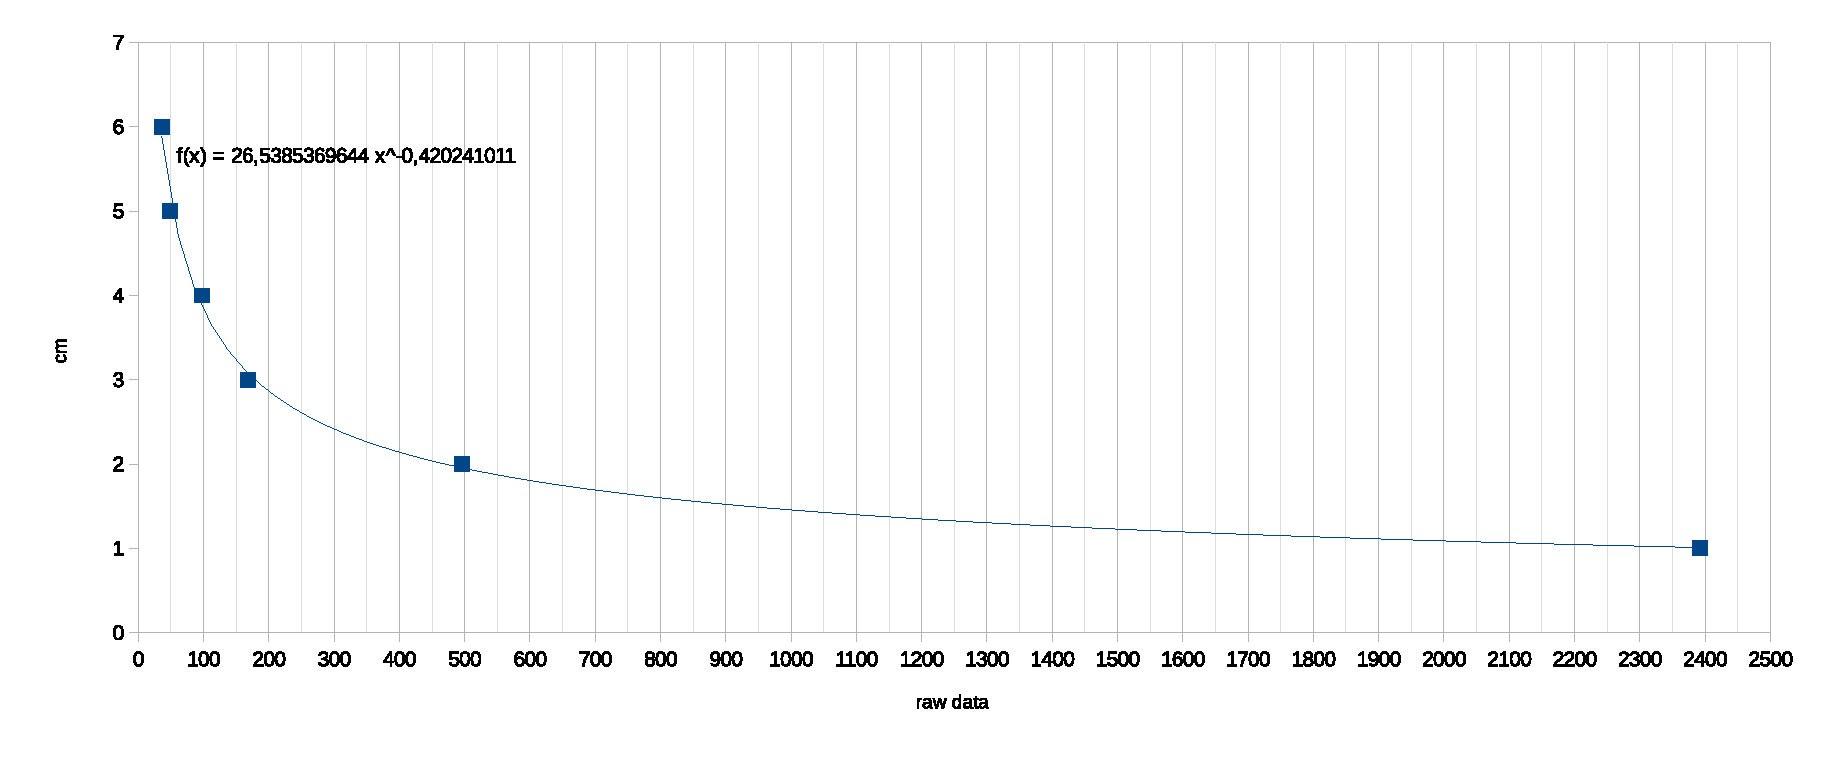
\includegraphics[width=\textwidth]{Proximitygraph.eps}
\label{fig:proxdata}
\caption{$x$-Axis: Raw data given by the proximity sensors. $y$-Axis: Measured
distance. The trend line function can be used to convert given proximity data
to an approximated distance to an obstacle.}
\end{figure}

\subsection{IR-Signals}
We assume that the IR-Signals are stable and originate from the victim only.

\teststrat{IR-Stabilization}{
    The IR-Signal recognition should be robust against minor disturbances, e.g.
    due interferences with distant reflections or similar.
    Those unwanted peaks will be filtered out.
}{
    Tin Bot, LPS, Victim.
}{
    Integration test: When there is no clear line of sight between the Tin Bot
    and the victim, no LED should light up.
}{
    Correct overall behavior, because this is subject of own test strategies.
}

\teststrat{IR Anti Reflection}{
    There are not supposed to be elements around the maze reflecting the IR
    signals unwantedly. Therefore, we coated the borders in cellular rubber
    absorbing signals rather than reflecting them. 
}{
    Tin Bot, maze, spectators, borders.
}{
    Integration Test: 
    The Tin Bot is placed in the maze and turned on, but not
    started. In this mode, it reports incoming and deemed-valid signals using
    its LEDs. 

    The victim is turned on and moved around in the maze. There should not be
    any lit LEDs other than the expected ones.
}{
    Correct overall behavior, because this is subject of own test strategies.
}

\subsection{Fence}
Moreover, since the Tin Bots do not have access to ground sensors, we ensured
the environment to be a safe playground.

\teststrat{Fence}{
    The fences have to make sure that the Tin Bot will not fall off the table.
}{
    Tin Bot, Maze, LPS.
}{
    Unit test: Send move signal to Tin Bot and let it run towards the table's
    edge. \textbf{Caution:} Make sure the Tin Bot will be caught if the test
    fails.
}{
    Correct overall behavior, because this is subject of own test strategies.
}

\section{Actuators}

The actuators are tested in a most isolated environment.

\teststrat{Motors}{
    When setting the appropriate register values, the E-Puck is supposed to
    start moving.
}{
    Tin Bot, LPS, debug monitor.
}{
    Unit Test: Turn on the Tin Bot, setup the LPS. Make sure a connection
    between all components is established. Send a signal to the E-Puck setting
    the respective registers values. Ensure that the E-Puck starts moving.
}{
    Loss of packets due to Bluetooth problems are not tested, neither are faulty
    registers and memory. Such faults, however, become evident very quickly.
}

\teststrat{LEDs}{
    When setting the appropriate register values, the LEDs are supposed to
    light up.
}{
    Tin Bot, LPS, debug monitor.
}{
    Unit Test: Turn on the Tin Bot, setup the LPS. Make sure a connection
    between all components is established. Send a signal to the E-Puck setting
    the respective registers values. Ensure that the E-Puck starts triggering
    the LEDs.
}{
    Loss of packets due to Bluetooth problems are not tested, neither are faulty
    registers and memory. Such faults, however, become evident very quickly.
}

\end{document}